
% This LaTeX was auto-generated from an M-file by MATLAB.
% To make changes, update the M-file and republish this document.

\documentclass{article}
\usepackage{graphicx}
\usepackage{color}
\usepackage{listings}
\usepackage[framed]{mcode}
\usepackage{fullpage}
\usepackage{amsmath}
\usepackage[utf8x]{inputenc}
\usepackage{import}
\usepackage{setspace}
\usepackage{hyperref}
\definecolor{lightgray}{gray}{0.5}
\setlength{\parindent}{0pt}

\begin{document}

    
    
%\section*{}


\title{BE 521: Homework 0 Questions\\{\normalsize Introduction}\\{\normalsize Spring 2021}}
\author{15 points}
\date{Due: Thursday 1/28/2021 11:59 PM}
\maketitle
\textbf{Objective:} Working with the IEEG Portal, basic MATLAB commands, publishing LaTeX


\section{Unit Activity (15 pts)}
The dataset \texttt{I521\_A0001\_D001} contains an example of multiunit human iEEG data recorded by Itzhak Fried and colleagues at UCLA using 40 micron platinum-iridium electrodes.
Whenever you get new and potentially unfamiliar data, you should always play around with it: plot it, zoom in and out, look at the shape of individual items of interest (here, the spikes). The spikes here
will be events appx. 5 ms in duration with amplitudes significantly greater than surrounding background signal.
\begin{enumerate}
 \item Using the time-series visualization functionality of the IEEG
 Portal find a single time-window containing 4 spikes (use a window width
 of 500 ms). The signal gain should be adjusted so that the spikes can be seen in entirety. Give a screenshot of the IEEG Portal containing the requested plot.  Remember to reference the LaTeX tutorial if you need help with how to do this in LaTeX. (2 pts)\\

Include screenshot:
\begin{lstlisting}
% 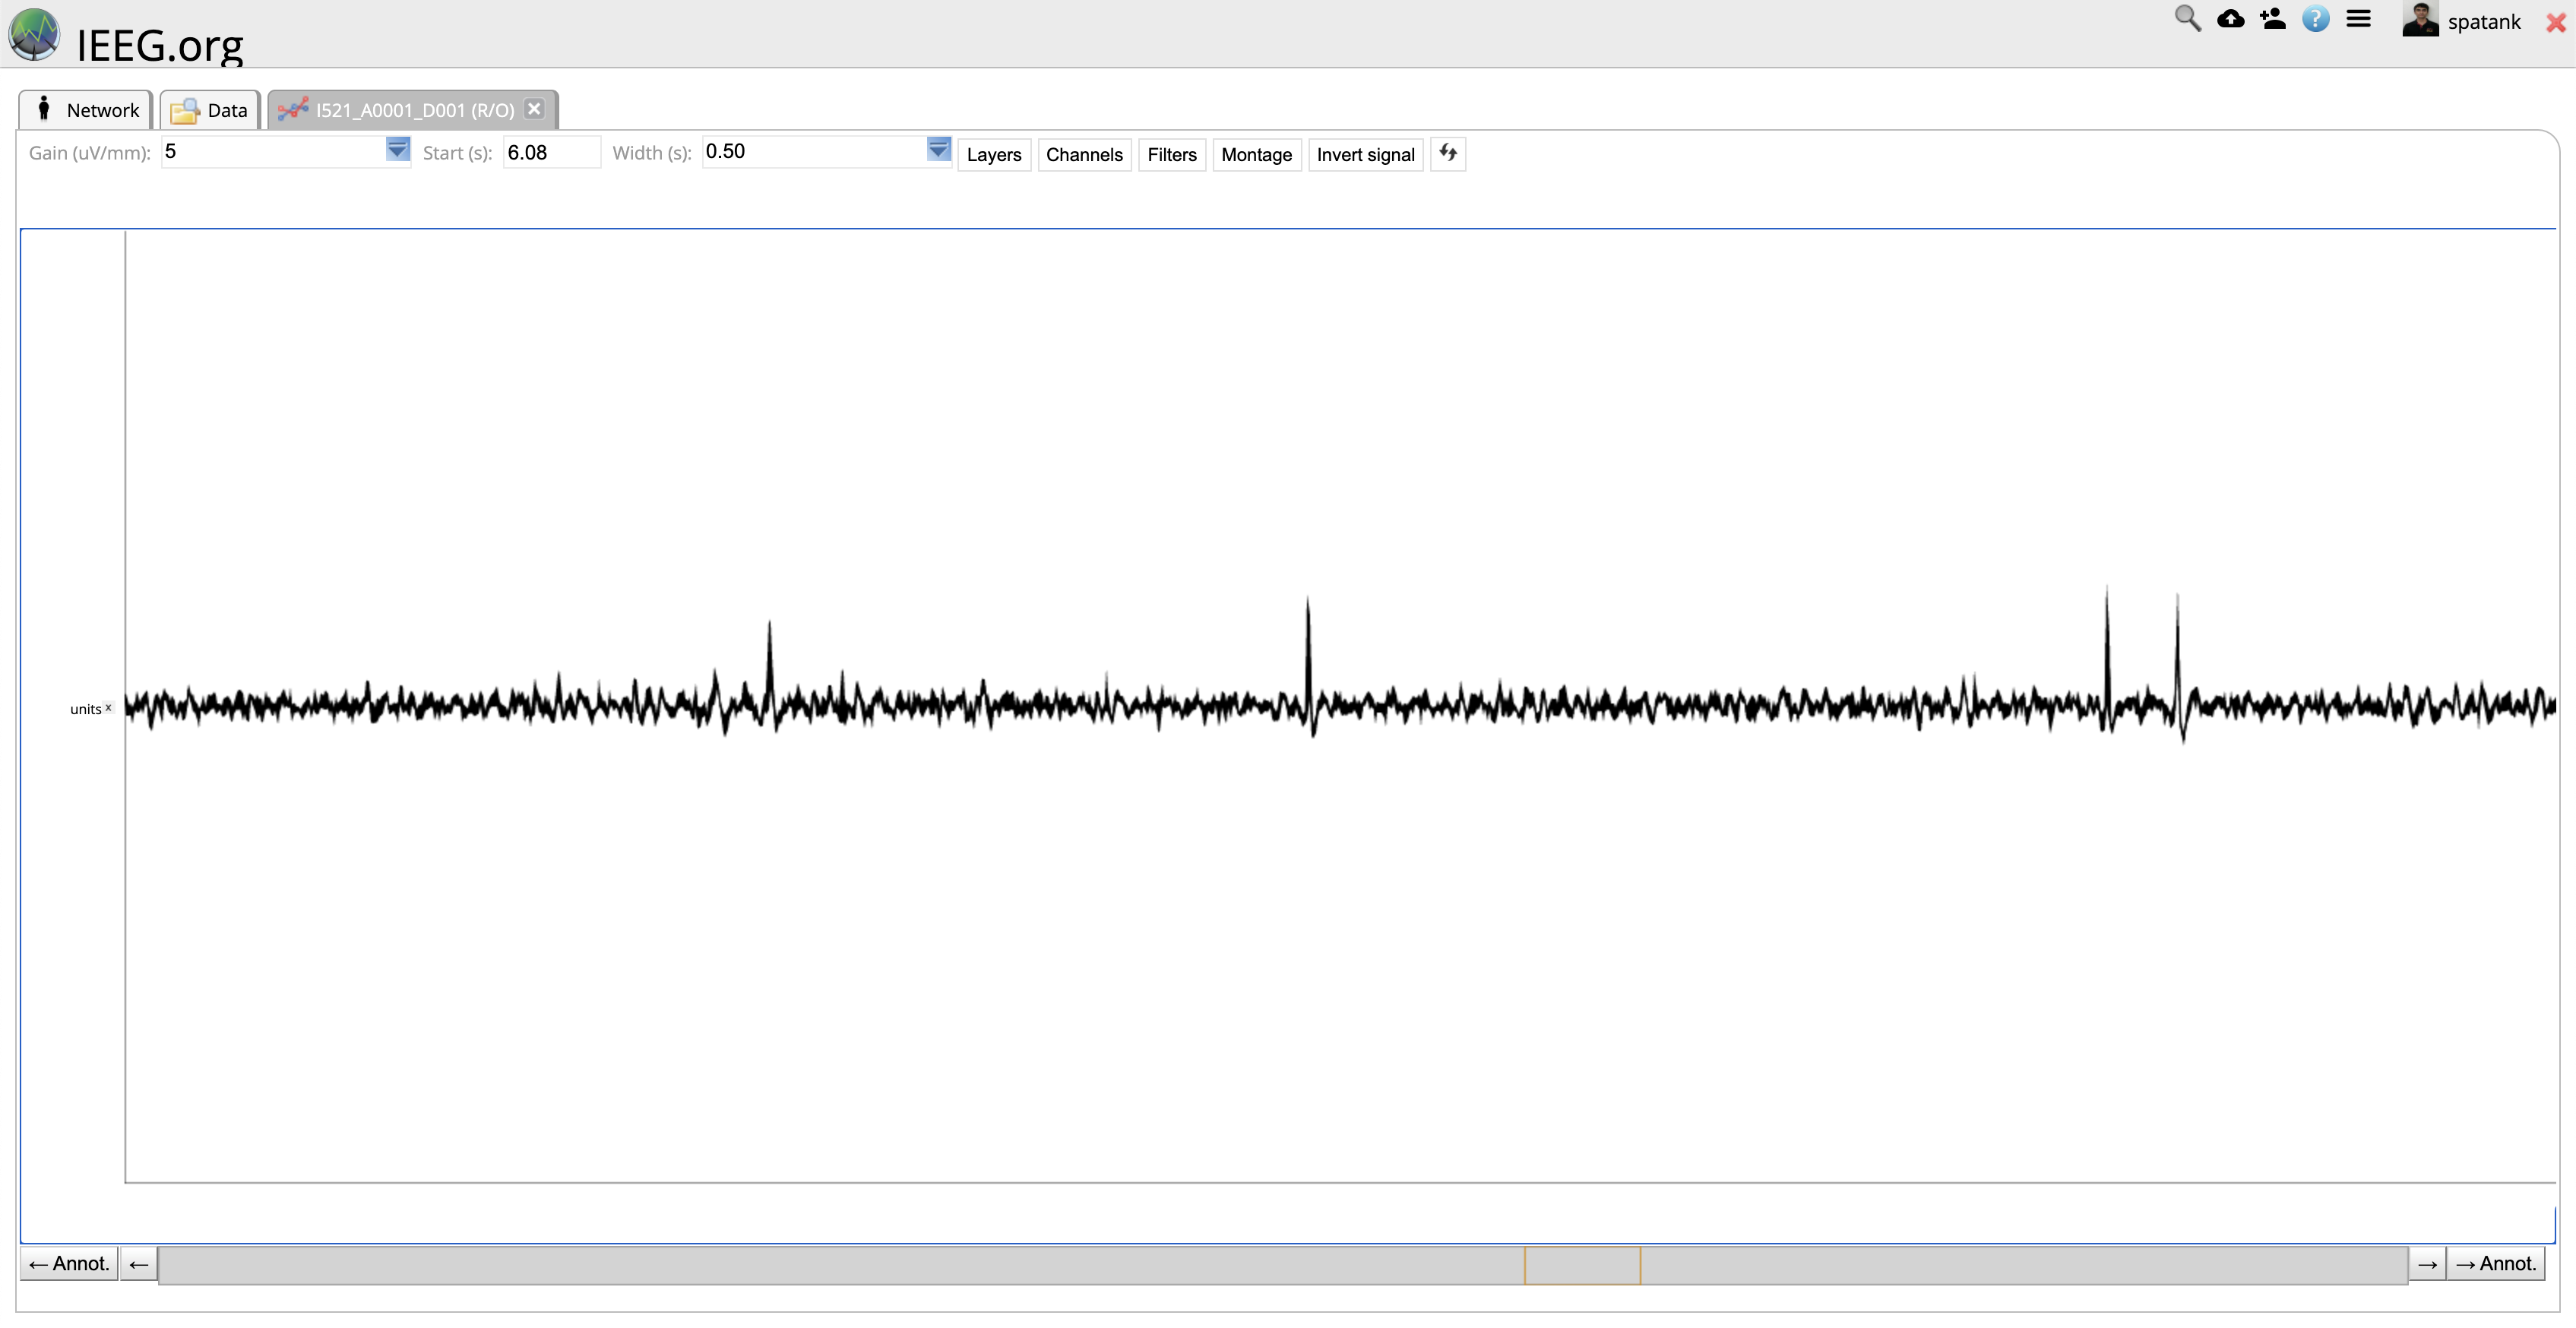
\includegraphics[scale=0.3]{screenshot.png}\\
\end{lstlisting}

 \item Instantiate a new IEEGSession in MATLAB with the
 \texttt{I521\_A0001\_D001} dataset into a reference variable called
 \emph{session} (Hint: refer to the IEEGToolbox manual, class tutorial, or the built-in \emph{methods} commands in the \emph{IEEGSession} object - i.e., \emph{session.methods}). Print the output of \emph{session} here. (1 pt)\\

ANSWER HERE
\begin{lstlisting}
cd('/Users/sppatankar/Developer/BE-521')
addpath(genpath('ieeg-matlab-1.14.49'))
addpath(genpath('Homework_0'))

% password_file = IEEGSession.createPwdFile('spatank', '***');

session = IEEGSession('I521_A0001_D001', 'spatank', 'spa_ieeglogin.bin')
\end{lstlisting}

\color{lightgray} \begin{lstlisting}IEEGSETUP: Adding 'ieeg-matlab.jar' to dynamic classpath
IEEGSETUP: Found log4j on Java classpath.
URL: https://www.ieeg.org/services
Client user: spatank
Client password: ****

session = 

  <a href="matlab:help('IEEGSession')">IEEGSession</a>:

      server: 'ieeg.org'
    userName: 'spatank'
        data: [1x1 IEEGDataset]

  <a href="matlab:methods(IEEGSession)">Methods</a>, <a href="matlab:IEEGObject.openPortalSite()">main.ieeg.org</a>

\end{lstlisting} \color{black}

 \item What is the sampling rate of the recording? You can find this
 information by exploring the fields in the \emph{session} data structure
 you generated above. Give your answer in Hz. (2 pts)\\

ANSWER HERE
\begin{lstlisting}
sampling_rate = session.data.sampleRate
\end{lstlisting}

\color{lightgray} \begin{lstlisting}
sampling_rate =

       32051

\end{lstlisting} \color{black}

 \item How long (in seconds) is this recording? (1 pt)\\

ANSWER HERE
\begin{lstlisting}
durationInUSec = session.data(1).rawChannels(1).get_tsdetails.getDuration;
durationInSec = durationInUSec/1e6
\end{lstlisting}

\color{lightgray} \begin{lstlisting}
durationInSec =

    10

\end{lstlisting} \color{black}

 \item
 \begin{enumerate}
    \item Using the \emph{session.data.getvalues} method retrieve the
    data from the time-window you plotted in Q1.1 and re-plot this data
    using MATLAB's plotting functionality. Note that the amplitude of the EEG signals from the portal is measured in units of $\mu V$ (microvolts), so label your y-axis accordingly.
    (NOTE: Always make sure to include the correct units and labels in your plots. This goes for the rest of this and all subsequent homeworks.). (3 pts)\\

ANSWER HERE
\begin{lstlisting}
start_time = 6.08;
window_size = 0.5;
channel_id = 1;
data_window = session.data.getvalues(start_time * 1e6, window_size * 1e6, channel_id);

figure;
plot(start_time:1/sampling_rate:start_time+window_size, data_window);
xlabel('Time (s)');
ylabel('\muV');
title('Channel 1 Signal');
\end{lstlisting}


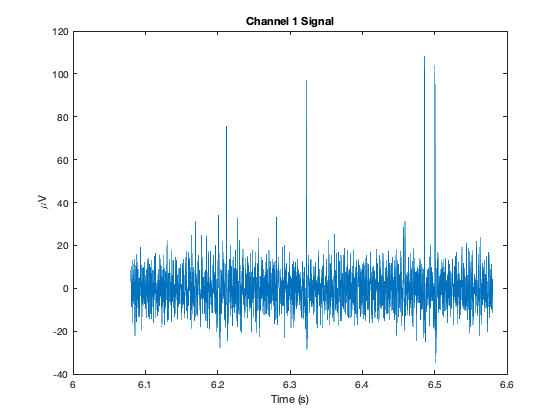
\includegraphics [width=5in]{spatank_hw0_01.png}

	\item Write a short bit of code to detect the times of each spike peak
	(i.e., the time of the maximum spike amplitude) within your
	time-window. Plot an 'x' above each spike peak that you detected superimposed on the plot from Q1.5a. (Hint: find where the slope of the signal changes from positive to negative and the signal is also above threshold.) (4 pts)\\

ANSWER HERE
\begin{lstlisting}
threshold = 50;
inds_df_2 = diff(diff(data_window) < 0);
inds_thresh = data_window(2:end-1) > threshold;
inds = find(inds_df_2 .* inds_thresh);

figure;
hold on
plot(start_time:1/sampling_rate:(start_time+window_size), data_window);
plot(start_time + (inds/sampling_rate), data_window(inds + 1), 'rx')
hold off
xlabel('Time (s)');
ylabel('\muV');
title('Channel 1 Signal');
\end{lstlisting}


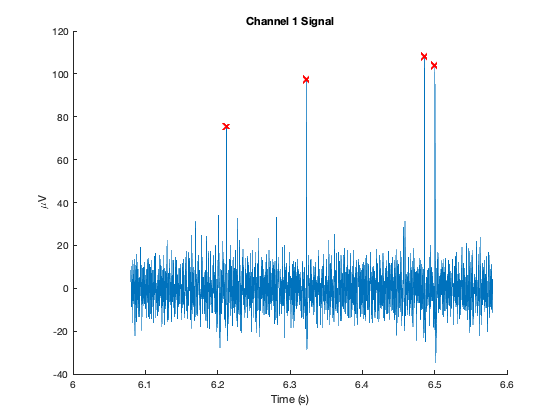
\includegraphics [width=5in]{spatank_hw0_02.png}

	\item How many spikes do you detect in the entire data sample? (1 pt)\\

ANSWER HERE
\begin{lstlisting}
data = session.data.getvalues(1, 10 * 1e6, channel_id);
inds_df_2 = diff(diff(data) < 0);
inds_thresh = data(2:end-1) > threshold;
inds = find(inds_df_2 .* inds_thresh);
num_spikes = length(inds)
\end{lstlisting}

\color{lightgray} \begin{lstlisting}
num_spikes =

    32

\end{lstlisting} \color{black}

\end{enumerate}
	\item Content Question - In the assigned reading, you
  learned about different methods to obtain and localize neural signals for BCIs.
  Describe the naming convention for the International 10-20 system for EEG recording. In your own words, what do the
	letters refer to and what can you infer from the parity (even vs. odd)
	of the number at a given site? (1 pt)\\

ANSWER HERE The first letter of an electrode's name denotes the region of the brain from which it records signals. Fp stands for pre-frontal, F for frontal, C for central, P for parietal, O for occipital, and T for temporal. These are appended to with numbers that denote which side of the head the electrode is placed at. Odd numbered electrodes are placed on the left-hand side of the skull, and even numbered electrodes on the right-hand side. Electrodes placed along the nasion-inion axis do not take a number, instead taking the letter z.

\end{enumerate}




\end{document}
    
